\chapter{Avaliação de Capacidade}
\label{chap:processo}
% ----------------------------------------------------------
Este capítulo apresenta uma proposta de processo de avaliação de capacidade
que visa a buscar as Configurações de menor preço capazes de executar uma determinada 
Carga de Trabalho. Esse processo foi implementado como parte de um sistema 
computacional ao qual demos o nome de \emph{Cloud Capacitor} e que descreveremos 
no capítulo seguinte.  

Antes de descrever o processo, é preciso que seja apresentado um 
conjunto de definições e terminologias que baseiam o entendimento da 
construção do trabalho e também a avaliação dos resultados, bem como a eficiência 
e eficácia da solução proposta. Os conceitos aqui explicitados são tomados de 
forma a permitir um estudo agnóstico quanto a aplicações, plataformas e provedores
utilizados durante a execução das ferramentas desenvolvidas neste trabalho.

\section{Definições e Terminologias}
Apresentamos a seguir as definições que permeiam o conhecimento necessário para 
a análise dos problemas estudados e soluções propostas. Mostramos também as 
terminologias ou nomenclaturas que criamos para designar esses conceitos a fim 
de facilitar a comunicação e o entendimento por parte do leitor.

\subsection{Aplicação sob Teste}
A Aplicação sob Teste é um sistema computacional, possivelmente implementado em 
arquitetura multicamadas, para o qual se deseja observar o comportamento em um 
ambiente de computação em nuvem e ao qual estão ligadas uma ou mais Métricas de 
Desempenho.

\subsection{Métrica de Desempenho}
Uma característica ou comportamento mensurável de forma automatizada e 
comparável a um Valor de Referência capaz de indicar o grau de sucesso de uma 
execução da Aplicação. Ex. tempo de resposta, quadros por segundo, etc. Métricas 
podem ser minimizáveis ou maximizáveis, a depender do objetivo da métrica quanto 
ao resultado desejado. Por exemplo, “tempo de resposta” é uma métrica 
minimizável, uma vez que geralmente se deseja que uma Aplicação responda a uma 
requisição com o menor tempo de resposta possível nos resultados. Contrariamente, 
uma métrica “quadros renderizados por segundo”, no domínio da computação gráfica, 
é uma métrica maximizável, pois quanto mais quadros são renderizados por unidade 
de tempo, maior a qualidade percebida pelo usuário.

\subsection{Valor de Referência de Desempenho ou SLA}
Um valor predefinido como minimamente aceitável como resultado apresentado por 
uma Métrica após uma Execução da Aplicação sob Teste. Este valor, também 
referenciado neste trabalho como SLA (Service Level Agreement), serve como base 
de comparação para que se classifique a Aplicação como capaz de ser executada 
em um determinado arranjo de máquinas virtuais e sob uma determinada Carga de
Trabalho a ela imposta.

\subsection{Provedor}
Consideramos neste trabalho a figura do provedor como representando uma empresa 
que fornece infraestrutura computacional como serviço cobrado financeiramente 
por fração de tempo de utilização. Alguns provedores fornecem conjuntamente a 
modalidade de plataforma como serviço. Nós, porém, não estamos considerando essa 
modalidade neste trabalho, interessando-nos apenas os serviços de infraestrutura, 
notadamente a disponibilização de máquinas virtuais.

\subsection{Tipos de Máquinas Virtuais}
Provedores costumam classificar as máquinas virtuais fornecidas conforme suas 
características, de modo a manter uma linha de produtos discreta e finita. 
Normalmente essa classificação se dá em termos de quantidade de memória RAM, 
quantidade de espaço em disco e capacidade computacional, neste caso, quer seja 
em termos relativos a um valor padrão tomado como base, quer seja em termos 
absolutos, como número de CPUs virtuais.

\subsection{Categorias de Máquinas Virtuais}
\label{subsec:definicoes_categorias}
Tipos de Máquinas Virtuais podem ser agrupados em Categorias, conforme suas 
características físicas, plataforma e/ou arquitetura de hardware e a natureza do 
uso a que se destinam. Dentro de uma mesma Categoria, os Tipos de Máquinas 
Virtuais variam apenas na quantidade de cada um dos recursos especificados para 
a Categoria e no preço cobrado pelo uso das máquinas virtuais.

Como exemplo, podemos citar uma Categoria de máquinas destinadas a armazenamento 
de arquivos, onde as máquinas devem privilegiar o espaço de armazenamento em 
massa. Dentro dessa categoria, a principal diferença entre os Tipos de Máquinas 
Virtuais se dá em função da quantidade de espaço em disco disponibilizado, 
enquanto características como memória RAM e CPU teriam pequenas variações. 
Outras Categorias podem enfatizar o consumo de banda de rede ou processamento 
paralelo de alto desempenho.

\subsection{Configurações}
Chamamos de Configuração um conjunto de máquinas virtuais pertencentes ao mesmo 
Tipo de Máquinas Virtuais e, portanto, de uma mesma Categoria. Configurações são
usadas para implantar uma camada arquitetural da Aplicação sob Teste (apresentação, 
negócio, persistência, etc.) e representam o estado de uma determinada camada da 
aplicação quanto à sua escalabilidade, vertical ou horizontal.

Por exemplo, suponhamos avaliação do comportamento de uma Aplicação cuja camada de
negócios está implantada em arquitetura de cluster de servidores de aplicação. 
Variando a quantidade de máquinas que compõem esse cluster, obtemos diferentes níveis
de escalabilidade horizontal para os quais podemos avaliar o desempenho da Aplicação.
Agora, suponhamos que podemos usar uma, duas, três ou quatro máquinas em paralelo como
componentes do cluster da camada de negócios da Aplicação sob Teste. Assim, teríamos
então quatro Configurações diferentes, a primeira com uma instância na camada de negócio,
a segunda Configuração com duas instâncias, a terceira com três e a quarta com quatro 
instâncias de máquinas do mesmo Tipo de Máquina Virtual. A Aplicação sob Teste seria 
executada quatro vezes, cada uma das quais utilizando uma dessas Configurações. Os 
resultados dessas Execuções refletem o efeito da escalabilidade horizontal no desempenho
geral da Aplicação.

Analogamente, poderiam ser usadas Configurações criadas a partir de Tipos de Máquinas
Virtuais diferentes, umas mais potentes que as outras. A comparação dos resultados obtidos
nesse cenário nos dão insumos para avaliar o efeito da escalabilidade vertical sobre o
desempenho da Aplicação.

Os experimentos desenvolvidos e apresentados neste trabalho comparam 
implantações de diferentes Configurações em uma determinada camada da Aplicação 
sob Teste estudada. Isso permite, por exemplo, que sejam feitas avaliações como 
a viabilidade financeira da escalabilidade vertical face ao desempenho 
possivelmente obtido com a escalabilidade horizontal.

\subsection{Espaço de Implantação}
Chamamos de Espaço de Implantação o conjunto limitado de Configurações tomadas 
para execução da Aplicação sob Teste em uma sessão de avaliação.
 
Idealmente, uma Aplicação deveria ser testada sob todos os Tipos de Máquinas 
Virtuais fornecidos pelo Provedor (cobrindo todo o espaço de escalabilidade 
vertical) com o maior número possível de combinações de quantidade de instâncias 
(cobrindo o espaço de escalabilidade horizontal). Porém, se muitos Tipos de 
Máquinas Virtuais forem necessários e se o intervalo de número de instâncias 
solicitado for muito grande, o tempo de duração da sessão e o custo da muitas 
execuções podem se tornar proibitivos.

Assim, o processo de especificação de um Espaço de Implantação consiste em 
selecionar uma lista de Tipos de Máquinas Virtuais entre os oferecidos pelo 
Provedor e designar o melhor valor para o número máximo de instâncias que serão 
usadas na criação das Configurações. Isso faz com que ambos os espaços de 
escalabilidade vertical e horizontal sejam limitados, de forma a controlar 
melhor os custos e permitir que sejam executados testes mais objetivos e de 
acordo com a meta de Carga de Trabalho a ser atendida pela Aplicação.

\subsection{Carga de Trabalho}
A Carga de Trabalho, ou Workload, representa o tamanho da demanda que será 
imposta à Aplicação sob Teste em uma execução. A unidade de medida da Carga é 
dependente do domínio da Aplicação, como a duração do vídeo em uma aplicação
de transcodificação de arquivos multimídia ou o tamanho do arquivos de entrada
para uma aplicação de compactação de arquivos. Entretanto, para efeito deste 
trabalho, essa unidade de medida da Carga é irrelevante, uma vez que a 
responsabilidade pela execução dos testes e, por conseguinte, pela geração da 
carga, é delegada a um módulo à parte dentro do sistema de avaliação, como um
software de \emph{benchmarking}.

\subsection{Execução}
Dá-se o nome de Execução ao evento de utilização de uma Configuração para 
executar a Aplicação sob Teste submetida a uma determinada Carga de Trabalho. 
Dessa forma, a avaliação dos Resultados de uma Execução nos dará uma ideia de 
como a Aplicação responderá às requisições de certo número de usuários (Workload) 
após ser implantada num ambiente de nuvem com certo grau de escalabilidade 
horizontal (número de máquinas virtuais usadas). 

Tome-se como exemplo uma aplicação web muito comum, um blog. São requisições 
comuns a um blog o acesso à página principal, uma consulta às postagens de uma
categoria e o acesso a uma postagem específica. Agora, suponha-se uma Configuração
composta de três instâncias de máquinas virtuais do Provedor Rackspace, do Tipo 
"Performance 1", executando uma instalação do blog Wordpress, muito usado hoje em 
dia. Uma Execução dessa aplicação seria a imposição da Carga de Trabalho correspondente
a um conjunto de requisições disparadas por 100 usuários simultâneos sobre essa Configuração. 

Introduzidas as definições e formalizações, torna-se possível agora a especificação 
de uma lógica de manipulaçãoo das entidades e operações descritas. As próximas 
seções descrevem a proposta de um Processo de Avaliação de Capacidade por 
Inferência de Desempenho cujo objetivo é identificar as Configurações capazes
de executar uma Aplicação respeitando um certo SLA definido.

\section{Visão Geral do Processo}
\label{sec:processo_visao_geral}

O processo (Figura~\ref{fig:fig_processo_alto_nivel}) prevê um conjunto de
dados de entrada, ao menos uma execução da Aplicação sob Teste no ambiente de nuvem de infraestrutura almejado para 
hospedá-la e a análise do desempenho obtido pela Aplicação a partir 
de suas execuções. Com base nos dados de desempenho, o processo passa por diversos
pontos de decisão que podem levar a novas execuções da Aplicação em diferentes 
cenários. Ao final do processo, é fornecida como saída uma lista de Configurações, 
ordenadas por preço, capazes de executar a Aplicação sob cada uma das Cargas de 
Trabalho fornecidas como parte dos dados de entrada.

\begin{figure}[h]
  \begin{center}
    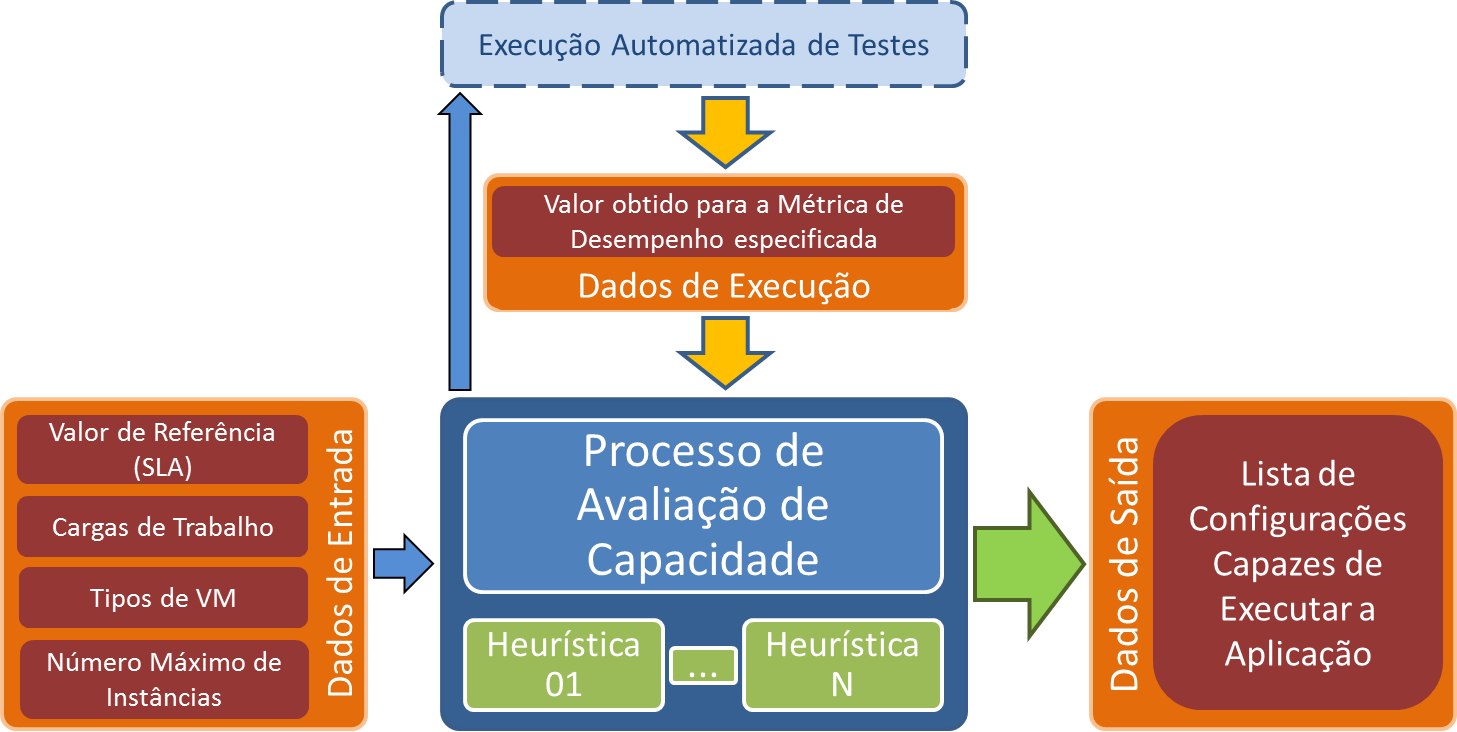
\includegraphics[scale=0.6]{img/processoAltoNivel}
  \end{center}
  \caption{\label{fig:fig_processo_alto_nivel}Visão geral do Processo de
  Avaliação de Capacidade}
\end{figure}

Este capítulo aborda em detalhes todas as fases do processo 
proposto, explicando quais são os dados de entrada necessários, as operações 
executadas pelo processo e quais as decisões pelas quais o processo tem que 
passar até determinar quais são as Configurações de menor custo capazes de 
executar a Aplicação.

\subsection{Dados de Entrada}

O principal parâmetro esperado pelo processo de avaliação de capacidade é o Valor
de Referência de Desempenho, ao qual também nos referimos como SLA 
(\emph{Service Level Agreement}). Esse valor será usado para determinar 
se a Aplicação atingiu os requisitos mínimos de desempenho exigidos, conforme
veremos na descrição do funcionamento do processo, mais adiante.

Além do SLA, o processo precisa também conhecer quais são as Cargas de Trabalho
para as quais o desempenho da Aplicação sob Teste deverá ser avaliado. Porém,
nem todas as Cargas de Trabalho serão impostas de fato à Aplicação. Isso vai 
depender do conjunto de decisões tomadas pelo processo com base na comparação do 
resultado obtido pela Aplicação com o SLA. Ainda assim, graças à sua característica 
de inferência de desempenho, o processo mostra resultados para todas as Cargas de 
Trabalhado informadas como parâmetro de entrada.

Para que o desempenho da Aplicação seja avaliado, é preciso que o processo conheça 
quais são as Configurações disponibilizadas no Provedor de nuvem para esse fim. 
Para isso, o processo deve ser alimentado com uma lista de Tipos de Máquinas Virtuais 
que serão utilizadas na execução da Aplicação, bem como a quantidade máxima de 
instâncias usadas para compor cada Configuração. Através desses dados o processo
passa a conhecer então o Espaço de Implantação disponível para os testes de 
desempenho, composto por uma lista de Configurações geradas a partir da lista de
Tipos de Máquinas Virtuais disponíveis e do número máximo de instâncias.

\subsection{Atividades Customizáveis}
O processo de avaliação de capacidade proposto é um processo extensível, do qual
fazem parte atividades customizáveis para as quais são delegadas funções de
cunho mais específico, como a comunicação com o Provedor de nuvem e a Aplicação sob Teste
para fins de orquestração do teste de desempenho, e também funções para as quais
é desejado um certo grau de flexibilidade a fim de tornar o processo mais adaptável,
como a escolha das Cargas de Trabalho e Configurações que serão usadas na execução
da Aplicação.

\subsubsection{Execução dos Testes de Desempenho}
Todas as atividades ligadas à rotina de execução da Aplicação, desde sua implantação,
passando pela criação e configuração das máquinas virtuais no ambiente do Provedor 
de nuvem, bem como pelo controle de inicialização e finalização dessas instâncias, 
serviços subjacentes como bancos de dados e filas, e a própria parametrização da 
execução e parada da Aplicação em si não fazem parte do escopo do processo. Este,
por sua vez, presume que os dados de resultado para cada execução estarão disponíveis
quando necessários. A maneira como esses dados serão de fato obtidos é
encapsulada pela implementação concreta desta atividade do processo.

%dependente da implementação concreta do processo e é irrelevante do ponto de
%vista do seu funcionamento.  

Portanto, o processo prevê a customização da atividade de Execução dos Testes,
que será responsável pelas ações necessárias à execução da Aplicação sob Teste no ambiente
alvo. A atividade customizada deverá conhecer os detalhes inerentes à comunicação com 
o Provedor e com a Aplicação sob Teste e, assim, ser capaz de ordenar a sua execução e 
coletar como resposta os dados de desempenho esperados pelo processo. Esse é um dos 
pontos de extensibilidade oferecidos pelo processo e sua implementação concreta está 
fora do escopo deste trabalho, cujo foco não está na automação de execução de testes 
de qualquer natureza, mas na análise dos dados resultantes dessa execução.

\subsubsection{Estratégias e Heurísticas}
\label{subsubsec:heuristicas}
De modo análogo à abordagem adotada em relação às atividades de execução dos
testes, as operações de seleção da Configuração sobre as quais a Aplicação
sob Teste será executada, bem como a seleção das Cargas de Trabalho a que ela 
será submetida durante sua execução, não são executadas diretamente pelo processo.
Nesse caso, são delegadas a uma atividade customizada que chamamos de Estratégia de 
Avaliação ou, simplesmente, Estratégia. Seu objetivo é permitir a aplicação de 
diferentes métodos para a escolha da melhor Configuração e/ou Carga de Trabalho 
mais adequada aos objetivos da avaliação de capacidade em curso e também ao perfil 
da Aplicação.

Como veremos na seção~\ref{sec:funcionamento_processo}, em diversas oportunidades
durante a execução do processo se faz necessária a seleção de uma Configuração de
maior ou menor capacidade. Do mesmo modo, em certos momentos o processo precisa
que uma Carga de Trabalho menor ou maior seja selecionada. A partir dessas escolhas
o processo é capaz de navegar no Espaço de Implantação submetendo a Aplicação sob
Teste a diferentes cenários de Cargas de Trabalho em diversas condições de capacidade
computacional.

Um problema relacionado à execução de testes de desempenho em ambientes de nuvem
é que o próprio teste implica num custo financeiro que pode ser bastante elevado
caso o Espaço de Implantação definido seja muito extenso. O mesmo se dá com 
relação à lista de Cargas de Trabalho. A fim de minimizar esse problema, este
trabalho propõe a técnica de inferência de desempenho explicada
detalhadamente na seção~\ref{subsec:processo_niveis_capacidade}, e através da
qual será possível eliminar grande parte das execuções reais da Aplicação
durante os testes, reduzindo assim o custo total da avaliação.

Porém, outro problema enfrentado na busca pela melhor Configuração capaz de executar 
uma Aplicação está justamente no momento de selecionar, dentre um conjunto de 
Configurações possíveis, qual a mais promissora a ser usada para uma execução real, 
dado que não é conhecido previamente o potencial computacional dessas Configurações.

A fim de solucionar esse problema, este trabalho introduz o conceito das 
Heurísticas de Seleção, que são abordagens a serem observadas no momento em que
a Estratégia de Avaliação deve escolher a próxima Configuração ou a próxima Carga 
de Trabalho. 

Foi definido um conjunto de 3 abordagens aplicáveis ao Espaço de Implantação,
ou seja, à escolha da próxima Configuração a ser testada, e outras 3 abordagens
aplicáveis à lista de Cargas de Trabalho. A combinação dessas abordagens dá origem
a 9 Heurísticas de Seleção, a saber:

\begin{description}
  \item[OO - Otimista/Otimista] \hfill \\ Visa Configurações menores e Cargas de Trabalho maiores
  \item[OC - Otimista/Conservadora] \hfill \\ Visa Configurações menores e Cargas de Trabalho intermediárias
  \item[OP - Otimista/Pessimista] \hfill \\ Visa Configurações e Cargas de Trabalho menores
  \item[CO - Conservadora/Otimista] \hfill \\ Visa Configurações intermediárias e Cargas de Trabalho maiores
  \item[CC - Conservadora/Conservadora] \hfill \\ Visa Configurações e Cargas de Trabalho intermediárias
  \item[CP - Conservadora/Pessimista] \hfill \\ Visa Configurações intermediárias e Cargas de Trabalho menores
  \item[PO - Pessimista/Otimista] \hfill \\ Visa Configurações e Cargas de Trabalho maiores
  \item[PC - Pessimista/Conservadora] \hfill \\ Visa Configurações maiores e Cargas de Trabalho intermediárias
  \item[PP - Pessimista/Pessimista] \hfill \\ Visa Configurações maiores e Cargas de Trabalho menores
\end{description}

Para um melhor entendimento de como as Heurísticas influenciam a navegação do 
processo entre as Configurações que compõem o Espaço de Implantação a ser explorado
e também entre as Cargas de Trabalho a serem impostas sobre a Aplicação, convém
observar a Figura~\ref{fig:heuristicas}.

\begin{figure}[hbt]
  \begin{center}
    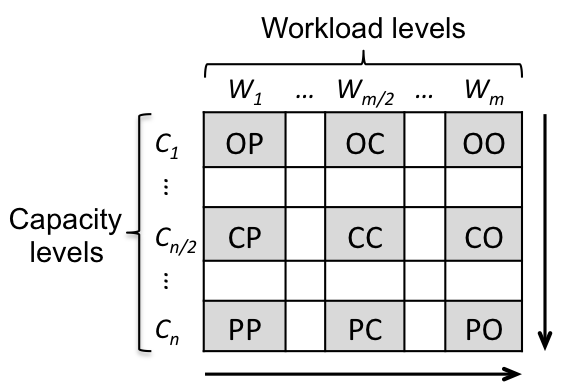
\includegraphics[scale=1]{img/heuristics}
  \end{center}
  \caption{\label{fig:heuristicas}Diagrama de Funcionamento das Heurísticas de Seleção}
\end{figure}

A imagem ilustra dois conjuntos dispostos em forma de matriz, um conjunto 
na vertical, formando as linhas, composto de $n$ Configurações $C_1 \ldots C_{n/2} 
\ldots C_n$ e um conjunto composto de $m$ Cargas de Trabalho $W_1 \ldots W_{m/2} 
\ldots W_m$, formando as colunas. As células dessa matriz mostram as Heurísticas
que selecionariam o par formado pela Configuração e pela Carga de Trabalho referentes
à linha e coluna da célula. Nessa representação das Heurísticas, a primeira letra
refere-se à abordagem usada para a escolha da Configuração e a segunda letra refere-se 
à abordagem usada na escolha da Carga de Trabalho.
 
Podemos ver, então, que as Heurísticas com abordagem Otimista escolherão Configurações 
mais próximas a $C_1$ e Cargas de Trabalho mais próximas a $W_m$. Por serem otimistas, essas 
abordagens consideram que máquinas menores são capazes de executar sob cargas 
mais severas.

Ainda com base na mesma imagem, vemos que as abordagens conservadoras se concentram
nas células intermediárias, conforme a descrição das Heurísticas. A Heurística
OC, otimista para Configurações e conservadora para Cargas, se concentra na 
primeira linha, ou seja, mais próxima de $C_1$, e nas colunas do centro, mais
próximas de $W_{n/2}$. Observação similar se faz para a Heurística PO, pessimista 
para Configurações e otimista para Cargas, concentrando-se nas últimas linhas e 
últimas colunas, ou seja, Configurações e Cargas maiores.

Voltando a tratar das Estratégias de Avaliação, estas serão responsáveis por efetuar
a escolha de Configurações e Cargas de Trabalho implementando a lógica prevista pelas
Heurísticas. Enquanto as Heurísticas são lógicas que indicam as proximidades onde 
deve ser feita a escolha de Configurações e Cargas, a Estratégia implementa de fato
um algoritmo que reflita o comportamento esperado pela ideia da Heurística.
 
A aplicação das Heurísticas de Seleção, através da implementação de Estratégias 
de Avaliação, está intrinsecamente ligada aos objetivos deste trabalho de estudar 
os efeitos da inferência de desempenho na eficiência do processo de avaliação de 
capacidade para aplicações em ambientes de nuvem de infraestrutura. A inteligência 
das Heurísticas propostas, ou seja, sua capacidade de escolher corretamente as 
Configurações e Cargas de Trabalho, é determinante para o sucesso do processo e 
da técnica de inferência. A eficácia e efetividade da aplicação das heurísticas
é analisada no capítulo~\ref{chap:resultados}. 

\begin{figure}
  \begin{center}
    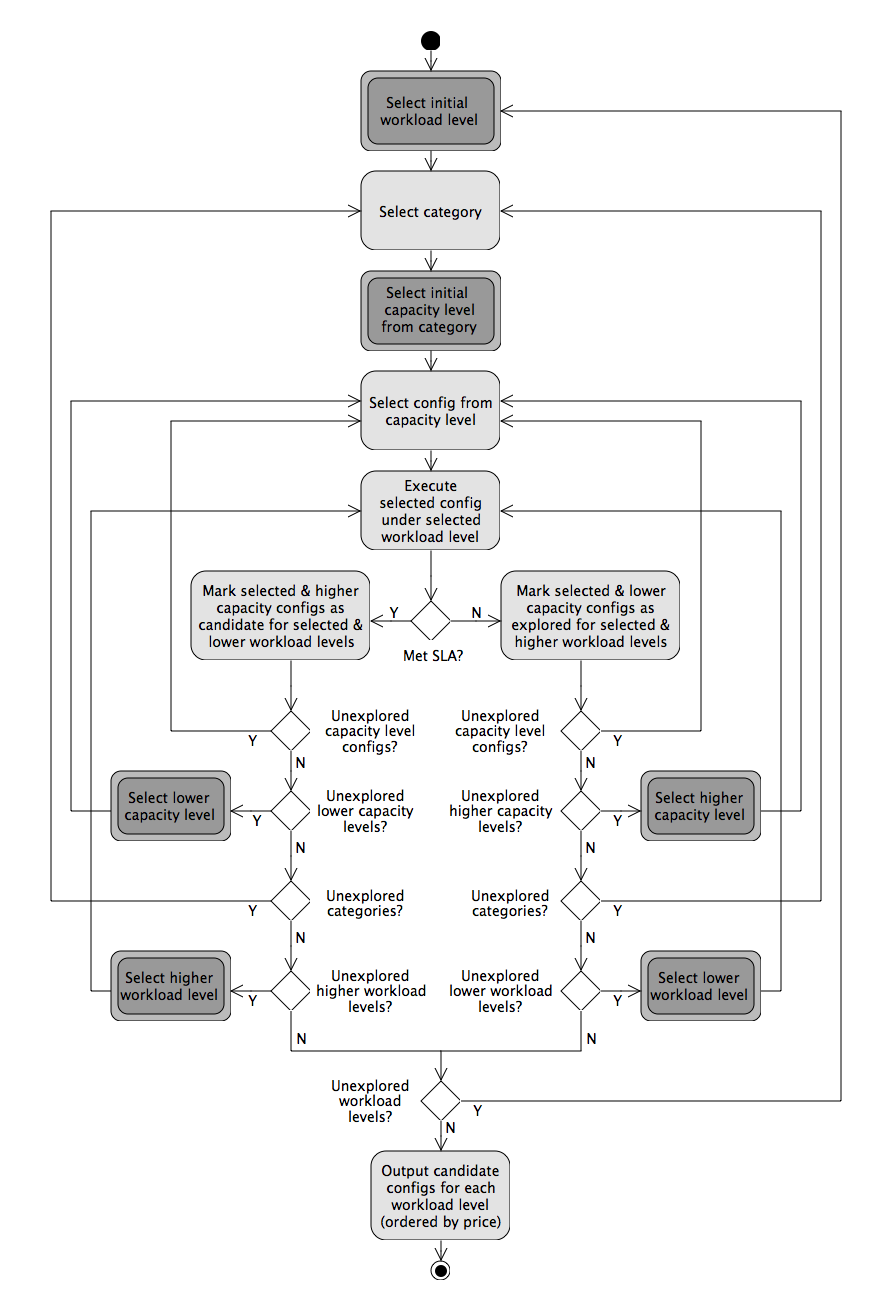
\includegraphics[scale=0.45]{img/capacity-planning-diagram-v13-mono}
  \end{center}
  \caption{\label{fig:fig_processo_aval_capacidade}Diagrama de Funcionamento do Processo de Avaliação de Capacidade}
\end{figure}

\section{Funcionamento do Processo}
\label{sec:funcionamento_processo}
Para efeito de entendimento do funcionamento geral do processo de avaliação de 
capacidade ora proposto, podemos abstrair temporariamente o comportamento das 
Heurísticas. Esta é, aliás, outra vantagem da abordagem adotada de 
delegação de funções específicas a atividades customizadas: além da flexibilidade e 
adaptabilidade, a abstração dessas operações torna mais fácil o entendimento, 
a descrição e a implementação concreta do processo.

Na Figura~\ref{fig:fig_processo_aval_capacidade}, os blocos em destaque representam
as operações que o processo espera que sejam executadas por uma Estratégia de 
Avaliação que implemente as Heurísticas propostas na seção anterior. Os outros 
blocos referem-se a ações comuns do próprio processo, executadas de maneira 
idêntica independentemente de qual seja a Aplicação sob Teste ou de qual seja a 
Estratégia de Avaliação usada. A delegação de funções para a atividade de Execução
de Testes não está destacada no diagrama e se dá no passo ``\emph{Executar
config sob nível de carga}'', situado aproximadamente no centro da figura.

\subsection{Operações iniciais}
\label{subsec:processo_operacoes_iniciais}
Uma vez tendo recebido os dados de entrada, o Processo tem seu início com o momento 
de escolher por onde começar a execução dos testes.

A primeira atividade desempenhada pelo Processo é a escolha da Carga de trabalho
inicial. A Estratégia é solicitada para realizar esta escolha que deve
seguir a orientação dada pela lógica da Heurística selecionada para 
a avaliação. Assim, será escolhido
um volume de carga maior se a Heurística for Otimista ou um volume menor se a
Heurística para Cargas de Trabalho for Pessimista. 

Depois de selecionar o nível de carga, o processo segue para selecionar a
Categoria. Conforme as definições apresentadas na Seção~\ref{subsec:definicoes_categorias}, 
os Tipos de Máquinas Virtuais oferecidos pelo Provedor são normalmente agrupados 
por Categorias, que reunem máquinas de propósito e atributos semelhantes. Dessa
forma, o Espaço de Implantação sobre o qual a avaliação de capacidade se dará está 
dividido em Categorias. O número de Categorias envolvidas na avaliação depende do 
conjunto de Tipos de Máquinas Virtuais selecionados pelo usuário e passados como
parte dos dados de entrada do Processo.

O Processo de Avaliação seleciona a primeira
Categoria de máquinas a ser explorada. O processo não especifica a ordem ou método 
dessa escolha, pois essa ordem não é importante uma vez que todas as Categorias 
presentes no Espaço de Implantação serão avaliadas. Conforme veremos no 
Capítulo~\ref{chap:capacitor}, a implementação de referência do Processo 
desenvolvida neste trabalho escolhe a primeira Categoria em ordem alfabética pelo
nome. Outras implementações do processo podem optar por outros métodos de
escolha.



\subsubsection{Níveis de Capacidade}
\label{subsec:processo_niveis_capacidade}
Dando continuidade à sequência de operações iniciais dentro do Processo de Avaliação 
de Capacidade, o próximo passo prevê que a Estratégia de Avaliação deve selecionar 
um Nível de Capacidade inicial. 

Níveis de Capacidade são um conceito criado para ajudar a estabelecer uma hierarquia 
sobre as relações de capacidade de processamento entre as diversas Configurações. 
Essa hierarquia de capacidade é válida apenas entre Configurações de uma mesma 
Categoria de Máquinas Virtuais. 

Para cada Categoria, o Nível ``um'' de Capacidade é composto apenas pela Configuração 
de menor preço dentro da Categoria. Um novo nível é criado com todas as Configurações 
para as quais é verdadeira a relação ``maior que''. Considera-se que uma 
Configuração $C_1$ é ``maior que'' uma outra Configuração $C_2$ se: 

\begin{enumerate}[label=\bfseries \alph*)]
\item ambas são formadas pelo mesmo Tipo de Máquina Virtual e $C_1$ possui 
número maior de instâncias do que $C_2$; ou
\item ambas são formadas pelo mesmo número de instâncias
e o Tipo de Máquina de $C_1$ possui mais CPU e mais memória que o Tipo de Máquina
de $C_2$.  
\end{enumerate}

Esse, então, passa a ser o Nível 
``dois'' e a lógica se repete daí em diante, tomando-se, para cada Configuração 
desse nível, as imediatamente maiores, formando um novo Nível. O procedimento 
continua até que todas as Configurações estejam devidamente classificadas em 
Níveis de Capacidade.

A Figura~\ref{fig_niveis_capacidade} mostra um pequeno exemplo, onde 6 Configurações,
pertencentes a duas Categorias distintas, foram classificadas em dois Níveis de 
Capacidade dentro de cada Categoria. Os retângulos representam as Configurações, 
com o texto indicando o nome do Tipo de Máquina Virtual utilizado e o número entre 
parênteses representando a quantidade de instâncias que compõem a Configuração. 
As setas que ligam as Configurações indicam a existência da relação de capacidade 
entre elas apontando da menor para a maior. A ausência de seta entre duas Configurações 
implica a impossibilidade de se afirmar uma relação de capacidade entre elas. 

\begin{figure}
  \begin{center}
    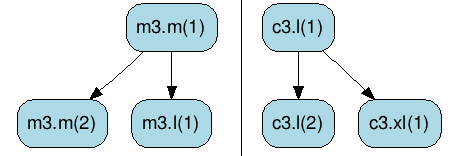
\includegraphics[scale=1]{img/exemplo-niveis-capacidade}
  \end{center}
  \caption{\label{fig_niveis_capacidade}Agrupamento de Configurações por Níveis de Capacidade}
\end{figure}

Assim, observando o Espaço de Implantação organizado por Categorias e classificado
hierarquicamente, a Estratégia deve selecionar, com base em uma das Heurísticas 
propostas na seção~\ref{sec:heuristicas}, um Nível de Capacidade inicial. As 
Configurações que fazem parte do Nível inicial escolhido são disponibilizadas 
para que a Avaliação proceda com a execução dos testes da Aplicação.

\subsection{Execução do Teste de Desempenho}
\label{subsec:processo_execucao}
Após a escolha da Carga de Trabalho inicial e do primeiro Nível de Capacidade a
ser avaliado, uma Configuração deve ser tomada a partir do Nível de Capacidade 
atual. Essa seleção não segue nenhuma regra específica, uma vez que todas as 
Configurações do Nível de Capacidade devem ser avaliados, ainda que por meio da técnica de 
Inferência de Desempenho, vista adiante.
 
Executa-se, então, a Aplicação sob Teste, impondo-se a ela a Carga de Trabalho 
selecionada, e analisa-se o resultado dessa execução. Nesse ponto o Processo se 
bifurca, atingindo seu primeiro ponto de decisão.

Esse é o momento em que a técnica de Inferência, conforme propomos neste trabalho,
será aplicada. A análise do Resultado obtido, mais especificamente do valor atribuído
à Métrica de Desempenho avaliada, comparado ao parâmetro do Valor de Referência, 
ou SLA, define se a Aplicação é ou não capaz de atender à demanda imposta pela
Carga de Trabalho. Vejamos a seguir uma explanação mais detalhada a respeito das
inferências que sucedem essa análise.  

\subsubsection{Inferência de Desempenho}
O processo de Inferência de Desempenho acontece logo após a análise comparativa
do Resultado, conseguinte a uma execução real da Aplicação sob Teste em uma 
Configuração, que foi tomada a partir de um Nível de Capacidade previamente 
selecionado. Durante essa execução, foi imposta sobre a Aplicação uma Carga de 
Trabalho, também previamente selecionada.

Observando o diagrama da Figura~\ref{fig:fig_processo_aval_capacidade}, podemos 
ver, bem ao centro, o ponto de decisão que define o sucesso ou o fracasso da 
Aplicação em atingir o SLA exigido. 

Se o desempenho da Aplicação satisfaz o SLA proposto, o Processo considera que a
Configuração é capaz de executar sob a Carga de Trabalho imposta e diz que a 
Configuração atual (sobre a qual a Aplicação acabou de ser executada) deve ser
assinalada como uma Configuração Candidata.

Neste ponto, a técnica de Inferência de Desempenho é aplicada e, como vemos
no texto do diagrama do Processo, todas as Configurações maiores que a atual também
são assinaladas como Candidatas. Ora, se identificamos que uma certa Configuração
consegue executar a Aplicação sob uma certa Carga de Trabalho, é intuitivo o 
pensamento de que qualquer Configuração que possua maior poder computacional 
também seja capaz de executar a mesma Aplicação sob a mesma Carga de Trabalho.

Assim, usando a representação do Espaço de Implantação conforme descrito na
Seção~\ref{subsec:processo_niveis_capacidade}, o Processo assinala como candidatas
todas as Configurações para as quais, direta ou indiretamente, a Configuração 
atual aponte uma seta, ou seja, todas as Configurações ``maiores que'' a Configuração
atual. 

Mas a técnica de Inferência ainda vai mais longe. Sabendo que as Configurações
que acabaram de ser assinaladas como Candidatas são capazes de executar a Aplicação
sob a Carga de Trabalho atual, também é intuitivo concluir que Cargas de Trabalho 
menores, ou mais brandas, serão naturalmente atendidas.

Então, prosseguindo com a aplicação da Inferência de Desempenho, o Processo marca
a Configuração atual e todas as maiores que ela como Candidatas não só para a 
Carga de Trabalho atual, mas também para todas as Cargas inferiores à atual.

De volta ao ponto de decisão da análise do Resultado em relação ao SLA, caso o 
desempenho da Aplicação não satisfaça o SLA, o Processo considera que a 
Configuração não é capaz de executar sob a Carga de Trabalho atual. Assim, essa
Configuração é marcada como Rejeitada para tal Carga.

De forma coerente, a lógica de Inferência de Desempenho entende que, se dada 
Configuração não consegue executar uma Aplicação a contento sob uma certa Carga,
intuitivamente, as Configurações menores tampouco conseguirão. Assim, o processo
indica a marcação de todas as Configurações ``menores que'' a atual como 
Rejeitadas para a Carga de Trabalho atual. 

Ainda seguindo a Inferência de Desempenho, quando uma Configuração não consegue
atender a demanda de uma Carga de Trabalho, presume-se que também não consiga
atender a demandas maiores, ou mais severas. O Processo de Avaliação manda, então,
que a Configuração atual e todas as Configurações menores sejam também marcadas
como Rejeitadas para todas as Cargas de Trabalho maiores que a Carga atual. 

\begin{figure}[h]
  \begin{center}
    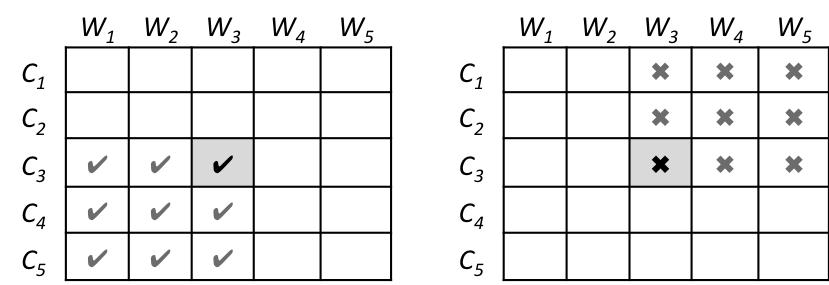
\includegraphics[scale=1]{img/inference}
  \end{center}
  \caption{\label{fig:fig_processo_inferencia}Inferência de Desempenho: Marcação de Configurações Candidatas e Rejeitadas}
\end{figure}

O efeito da aplicação da técnica de Inferência de Desempenho pode ser melhor
visualizado através da Figura~\ref{fig:fig_processo_inferencia}. A figura mostra 
duas situações: a da esquerda para o caso em que o SLA é satisfeito e a da direita 
caso o SLA não seja satisfeito. Em ambos os casos vemos uma célula central realçada, 
indicando que a Aplicação sob Teste foi executada na Configuração $C_3$ sob a 
Carga de Trabalho $W_3$. As células marcadas com $\sqrt{}$ mostram as Configurações
marcadas como Candidatas para as Cargas de Trabalho correspondentes. As células
marcadas com $\times{}$ representam as Configurações assinaladas como Rejeitadas.

Essa representação serve para demonstrar a contribuição da aplicação da técnica 
de Inferência na aplicação de testes de desempenho. Nesse exemplo, foram 
explorados 9 cenários diferentes, dados pelas combinações de Configurações e 
Cargas de Trabalho, mas apenas 1 execução real foi conduzida. Isso significa não
só que o tempo total gasto na Avaliação de Capacidade é reduzido, mas também o
custo financeiro envolvido nessa atividade. 

Mais adiante neste capítulo, expandiremos essa representação para mostrar a ação
da Inferência de Desempenho após várias iterações do laço compreendido pelo 
Processo de Avaliação. Por hora, continuemos com a descrição dos passos seguintes.

\subsection{Seleção dos Próximos Cenários}
\label{subsec:selecao_cenarios}
Passada a fase de Inferência de Desempenho, o processo segue seu caminho, tomando
as decisões que levarão à seleção dos cenários seguintes a serem avaliados quanto
à sua capacidade.

O ponto de decisão que sucede a marcação das Configurações Candidatas ou Rejeitadas
checa se existem Configurações pertencentes ao atual Nível de Capacidade cujas 
execuções ainda não tenham sido avaliadas para a Carga de Trabalho atual. Se 
existirem, o Processo volta ao passo de seleção de uma Configuração a partir do 
Nível de Capacidade e uma nova execução é solicitada.

Se não existirem Configurações inexploradas para a Carga de Trabalho atual no
Nível de Capacidade corrente, o Processo buscará por um Nível de Capacidade que 
ainda não tenha sido completamente explorado. Se a Aplicação satisfez o SLA na 
execução anterior, a Estratégia deverá selecionar um Nível de Capacidade menor. 
Se o SLA não tiver sido atingido, a Estratégia tentará selecionar um  Nível de 
Capacidade maior. Depois de selecionado o próximo Nível de Capacidade, o laço do
Processo retorna ao ponto de seleção da próxima Configuração e outra execução 
acontece.
   
Novo ponto de decisão surge quando a Estratégia não encontra um Nível de 
Capacidade a ser explorado. Nessa situação, o Processo procura uma outra
Categoria dentro do Espaço de Implantação que ainda possua pelo menos uma
Configuração ainda não explorada para a Carga de Trabalho atual. Se houver,
o Processo retorna ao passo de seleção de um Nível de Capacidade dentro da
Categoria selecionada e nova execução será realizada.

Caso não haja uma outra Categoria com Configurações não avaliadas, atingimos
então um outro ponto de decisão, onde a Estratégia deve buscar uma Carga 
de Trabalho que não tenha sido avaliada. Se a execução anterior atingiu o SLA,
uma Carga de Trabalho maior será buscada. Caso contrário, a Estratégia tentará
uma Carga menor que a atualmente selecionada. Se a Estratégia obtiver sucesso
nessa escolha, o Processo dispara uma nova execução da Aplicação com a Configuração
corrente e sob a Carga de Trabalho que acabou de ser selecionada.

Porém, se a Estratégia não conseguir fornecer uma Carga de Trabalho segundo as 
restrições do Processo segundo a comparação do Resultado com o SLA, o Processo 
voltará ao passo inicial de seleção de Carga de Trabalho, que não tem qualquer 
restrição quanto a essa seleção. Tentará assim a escolha de uma Carga inexplorada
qualquer. Caso não seja encontrada nenhuma Carga de Trabalho inexplorada, significa
que não há mais nada a ser testado e o Processo é encerrado.

\subsection{Finalização da Avaliação}
Não tendo mais Configurações a serem testadas sob nenhuma Carga de Trabalho, o 
Processo é dado por concluído e sua finalização se efetiva pela apresentação de uma
lista que contém, para cada Carga de Trabalho, as Configurações capazes de executar
a Aplicação sob Teste, em ordem crescente de preço.

Por ``capazes de executar'', entenda-se como as Configurações para as quais o valor
obtido para a Métrica de Desempenho durante a execução da Aplicação sob determinada
Carga de Trabalho é menor ou igual ao valor definido para o SLA ou Valor de Referência
como um dos dados de entrada no início do Processo de Avaliação de Capacidade.

Embora essa seja a resposta final do processo, a contribuição real deste trabalho está
na maneira como chegamos a essa resposta, com redução de custo e tempo, e na precisão 
da resposta, ou seja, o nível de acerto atingido pelo Processo ao apontar as Configurações
Candidatas e Rejeitadas. Dados reais que comprovam a eficácia do 
Processo e da técnica de Inferência de Desempenho propostos são apresentados no
Capítulo~\ref{chap:resultados}, que trata dos experimentos realizados e analisa criticamente os resultados obtidos.

Para deixar mais clara essa contribuição, é explicado a seguir
como o Processo constrói a resposta final, demonstrando o rastreamento dos vários momentos
em que a técnica de Inferência de Desempenho é empregada e evidenciando a influência que
a utilização de diferentes Heurísticas exerce sobre a eficiência do Processo.

\begin{figure}
  \begin{center}
    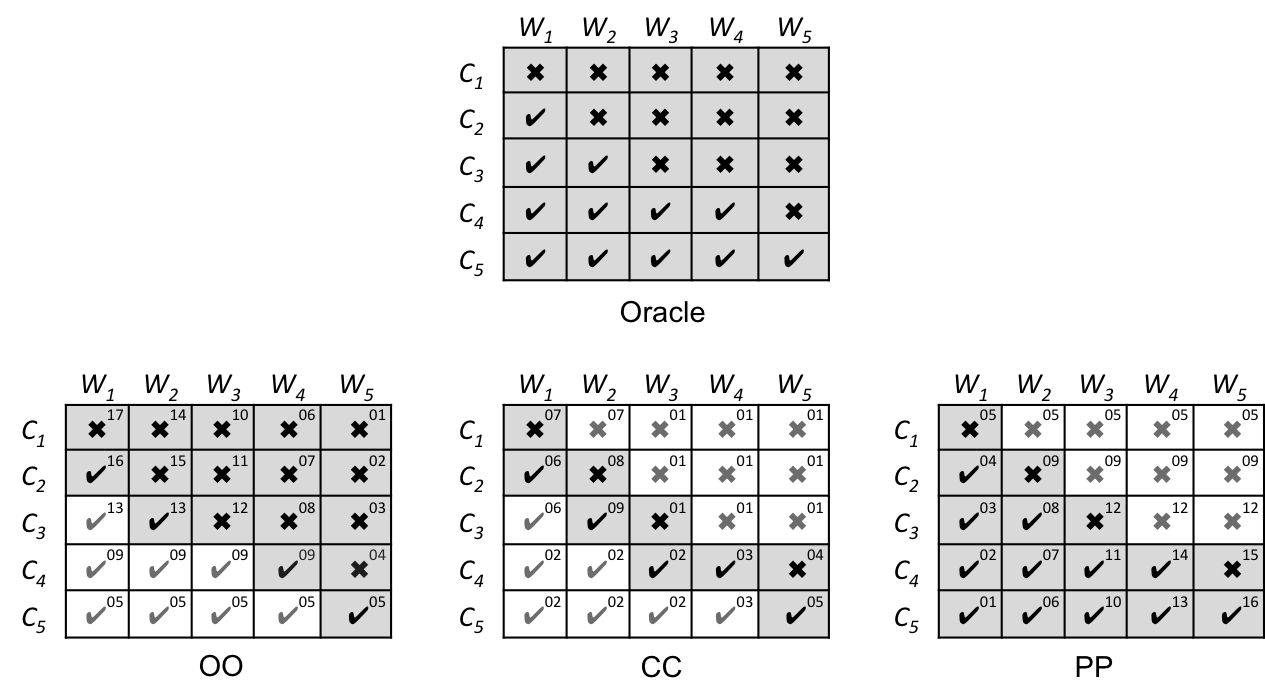
\includegraphics[scale=0.6]{img/traces}
  \end{center}
  \caption{\label{fig:fig_processo_traces}Rastreamamento da Execução das Heurísticas e Inferência de Desempenho}
\end{figure}

A Figura~\ref{fig:fig_processo_traces} mostra, nos quadros da parte inferior, 
o rastro de todas as iterações da execução do Processo de Avaliação com 3 
Heurísticas de Seleção distintas: Otimista/Otimista, Conservadora/Conservadora e 
Pessimista/Pessimista. O quadro da parte superior da imagem mostra o que seria o
resultado da execução real da aplicação em todos os cenários analisados, ou seja,
com todas as combinações de Configurações e Cargas de Trabalho. A essa 
representação damos o nome de Oráculo, por conter toda a informação real de
desempenho da Aplicação sob Teste considerada em cada cenário.

O Oráculo serve-nos de base de referência para a apuração da eficácia do Processo
e sua Inferência de Desempenho, ou seja, a precisão de acerto quanto a quais são
de fato as Configurações capazes de executar a Aplicação com desempenho que atenda
ao SLA. Além disso, com base no Oráculo, podemos também aferir qual a eficiência 
da Heurística utilizada na Avaliação, medindo a economia em número de execuções
reais e, por conseguinte, em tempo e custo financeiro da Avaliação.

As execuções reais são representadas nas figuras pelas células destacadas, mais 
escuras. As células marcadas com um $\sqrt{}$ indicam que a Aplicação atingiu um
desempenho que cumpre o SLA exigido para aquela combinação de Configuração e Carga
de Trabalho, ou seja, a Configuração é considerada Candidata para aquela Carga. As
células marcadas com um $\times$ mostram onde a Aplicação não conseguiu cumprir 
o SLA, ou seja, as Configurações Rejeitadas.

Dentro de cada célula nos quadros que mostram o comportamento das Heurísticas há
um número que indica em qual passo da iteração do processo a Configuração foi
marcada como Candidata ou Rejeitada. Alguns números são repetidos em várias células
e isso serve para mostrar a Inferência de Desempenho atuando. As células brancas
foram marcadas como Candidatas ou Rejeitadas por meio da técnica de Inferência no
passo denotado pelo pequeno número no canto da célula. Note-se que para as células 
destacadas os números não se repetem e demonstram a ordem de escolha das Configurações
pela Heurística para execução real da Aplicação.

Os exemplos apresentados na figura~\ref{fig:fig_processo_traces} mostram uma eficácia
de 100\%, ou seja, usando a Inferência, o Processo indicou com correção todas as
Configurações que, caso fossem testadas de fato, com uma execução real da Aplicação,
teriam um desempenho dentro do SLA esperado. A imagem mostra, ainda, que, para a 
Aplicação fictícia considerada, a Heurística Conservadora/Conservadora foi a mais
eficiente, com apenas 9 execuções reais contra um potencial total de 25 execuções.
Supondo que o tempo de execução dos testes de desempenho da Aplicação é o mesmo 
em cada iteração, isso representa uma economia de 64\% no tempo de execução da
Avaliação de Capacidade em comparação com a execução de todos os cenários.

Outra contribuição trazida pelo emprego das Heurísticas de Seleção de
Configurações é a automação da decisão de por onde começar a execução dos testes. Quando se faz
necessária a análise do comportamento de uma aplicação qualquer em um determinado
ambiente, com dezenas ou até centenas de variações tanto do ambiente como dos 
volumes de demanda, a escolha de uma combinação inicial dessas variáveis é um
problema de difícil solução.

O emprego das Heurísticas de Seleção ajudam não só na escolha da Configuração e 
da Carga de Trabalho iniciais, mas também de qual a próxima combinação a ser 
testada e sempre visando ao menor custo de execução dessa avaliação.

O Capítulo~\ref{chap:resultados} irá mostrar os resultados obtidos
com o Processo de Avaliação proposto e descrito neste trabalho ao avaliar uma
Aplicação real em um ambiente também real de nuvem de infraestrutura. Serão apresentados
resultados de eficiência e eficácia do emprego da técnica de Inferência de Desempenho
e das Heurísticas de Seleção, comparando-as sob diversos SLAs.

\section{Resumo}
Este capítulo apresentou uma proposta de processo de avaliação de capacidade
cuja ideia chave é a inferência de capacidade de um recurso a partir dos dados 
reais de desempenho obtidos por um outro recurso semelhante, mas de capacidade
presumidamente menor ou maior.

Essa proposta de processo se apoia na hipótese de que é possível estabelecer uma
relação de capacidade entre os recursos disponibilizados por um provedor de nuvem
de infraestrutura. Com base nessa hipótese, definiu-se uma sequência de passos
que visam a identificar quais recursos são capazes de executar uma determinada 
aplicação sob determinados volumes de carga de trabalho com o menor número
possível de execuções reais da aplicação. Como resultado, o processo busca
a redução de custo e tempo normalmente envolvidos na atividade de avaliação de
capacidade dos recursos disponíveis na nuvem.

O Capítulo~\ref{chap:capacitor} a seguir apresentará uma visão mais concreta,
com a descrição do arcabouço de software desenvolvido neste trabalho como implementação de referência
para o processo proposto. Além disso, será utilizada uma aplicação web para
ilustrar o uso do processo de avaliação de capacidade
baseado em inferência de desempenho. 

%Essa aplicação foi usada para demonstração da criação de algumas Estratégias
% criadas e para a execução dos testes de eficácia e efetividade das técnicas propostas, bem como das próprias
%Estratégias, e cujos resultados apresentaremos no
% Capítulo~\ref{chap:resultados} mais adiante.
   
% ----------------------------------------------------------
